\chapter{Implementation}

\section{Agent}

The agent was constructed with this structure......

\section{Genetic Algorithm}

The genetic algorithm was performed by a Runner class, which could take an environment and the current generation as inputs to \_\_init\_\_.

The score for each agent per generation was not just it's reward from a single play-through of Space Invaders. Instead, per generation, each agent ``played'' Space Invaders N times. N varied throughout the testing process to speed up testing, however N was always in the range [5,20] and N will be specified whenever a figure is displaying a set of results. The score for each play-through was recorded, and then final score for the agent can be calculate using this equation: $0.4(median(r)) + 0.6(mean(r))$, where r is the set of scores for the agent. The median was used as the scores were often skewed by a large outlier which greatly affected the mean. This means the algorithm targets more consistent game playing. However, the mean is still useful to try to exploit certain large outliers if possible, or perhaps an agent produced good scores and bad scores at an even ratio, so the mean was used to continue evolving some of these agents. Just using the median often lead to slow improvements as the models would converge on the median score for the game, rather than trying to get a higher score.

Experiments were then performed to determine the optimal crossover and mutation rates. To perform these, the selected crossover operator was Option 1, and the selected mutation operator was Option 2. Figure \ref{fig:crmr}\footnote{While the key in this figure states that the green line is the media score, it is in fact the median score. Each of these graphs too a long time to produce and I did not notice till the end of producing all 4.} shows these results. It shows the best score from the set agents, as well as the mean and median of the set of scores per generation. For all of these results the environment was experienced 10 times per agent per generation. Furthermore, each experience was limited to 1 life to speed up testing. From these results, CR was chosen to be $0.4$, and then Initial MR was chosen to be $0.3$. Furthermore, these results did not converge after 20 generations, so that suggests that there is still improvements to be made.

\begin{figure}
  \centering
  \subfloat[CR = 0.3, Initial MR=0.2]{
  \begin{minipage}[c]{0.4\textwidth}
    \centering
    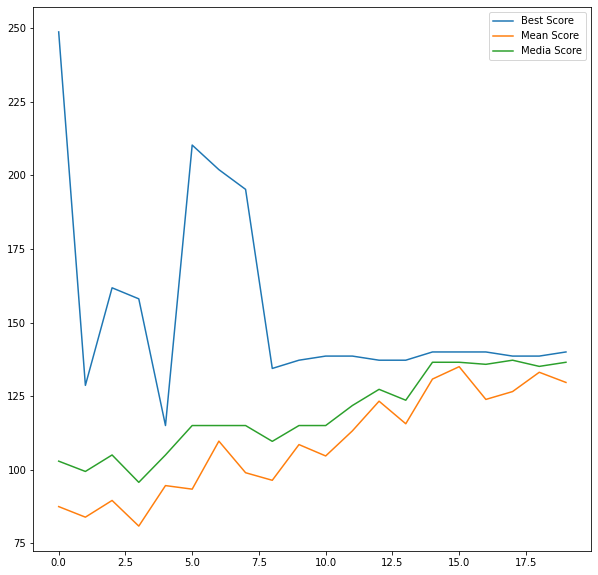
\includegraphics[scale=0.3]{images/03-cr-02-mr.png}
  \end{minipage}}
  \hfill
  \subfloat[CR = 0.2, Initial MR=0.4]{
  \begin{minipage}[c]{0.4\textwidth}
    \centering
    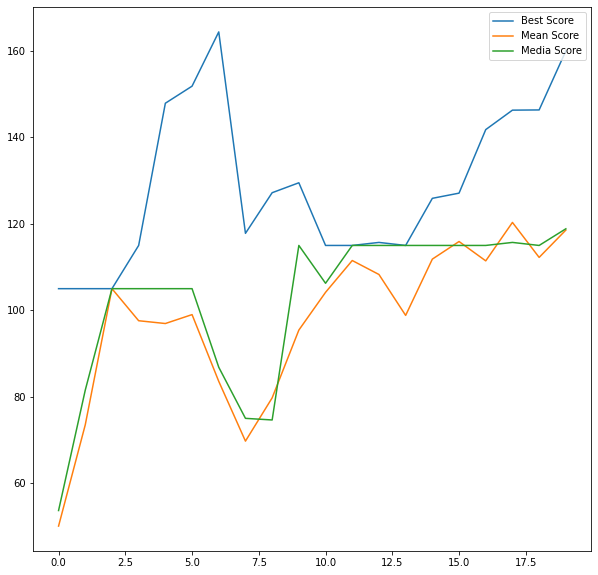
\includegraphics[scale=0.3]{images/02-cr-04-mr.png}
  \end{minipage}}
  \hfill
  \vfill
  \subfloat[CR = 0.4, Initial MR=0.3]{
  \begin{minipage}[c]{0.4\textwidth}
    \centering
    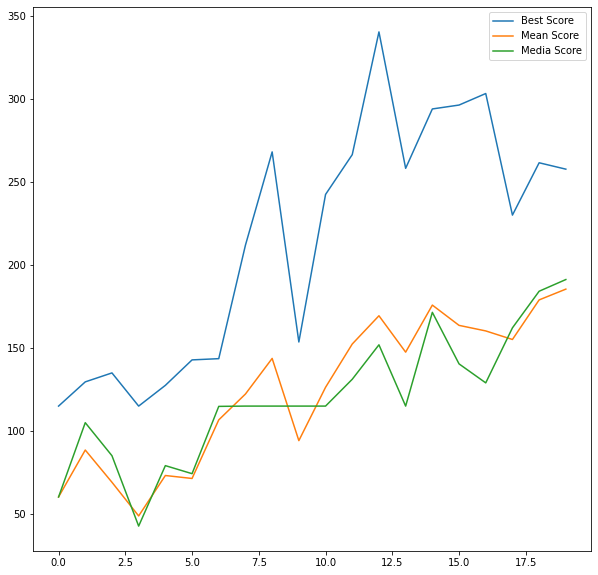
\includegraphics[scale=0.3]{images/04-cr-03-mr.png}
  \end{minipage}}
  \hfill
  \subfloat[CR = 0.4, Initial MR=0.2]{
  \begin{minipage}[c]{0.4\textwidth}
    \centering
    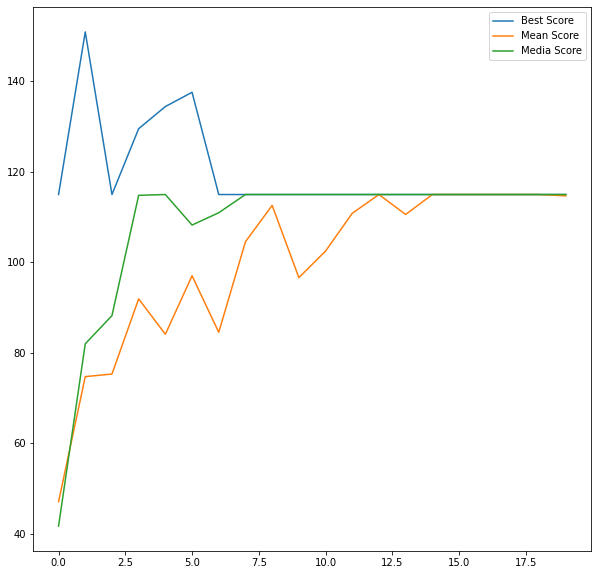
\includegraphics[scale=0.3]{images/04-cr-02-mr.png}
  \end{minipage}}
  \hfill
  \caption{CR and MR Testing}
  \label{fig:crmr}
\end{figure}

\paragraph{}


Using these determined rates both the mutation and crossover operators were tested. Initially, Option 2 for crossover was tested. This is where an entire layer was chosen to swap with both parents, if the chance was less than the crossover rate. The results of this coincided with my initial thoughts, and the models being using are likely too small for this option to be viable. Therefore, Option 1 was chosen, to randomly select an individual weight for crossover between two parents. For mutation, I tested the 3 different operators, the resulting output graphs can be see in Fig. N. For these results, the environment was experienced 5 times per agent per generation, and each experience was limited to 1 life. The total number of generations was limited to 5 due to time constraints. The final mutation operator was chosen to be .....


\section{Transfer Learning}

The transfer learning was implemented by initiating another runner class with a new environment and the resulting final generation of Space Invaders runner. The best model can then be selected and test on one experience of the new environment. This can be compared to 1 experience of an agent performing random actions on the same environment. The entire set of models can also be run through the genetic algorithm again to see how it long it takes for them to converge.
